\documentclass{article}
\usepackage{pgfplots}
\pgfplotsset{compat=1.17}

\begin{document}

\begin{figure}[h]
    \centering
    \begin{minipage}{0.45\textwidth}
        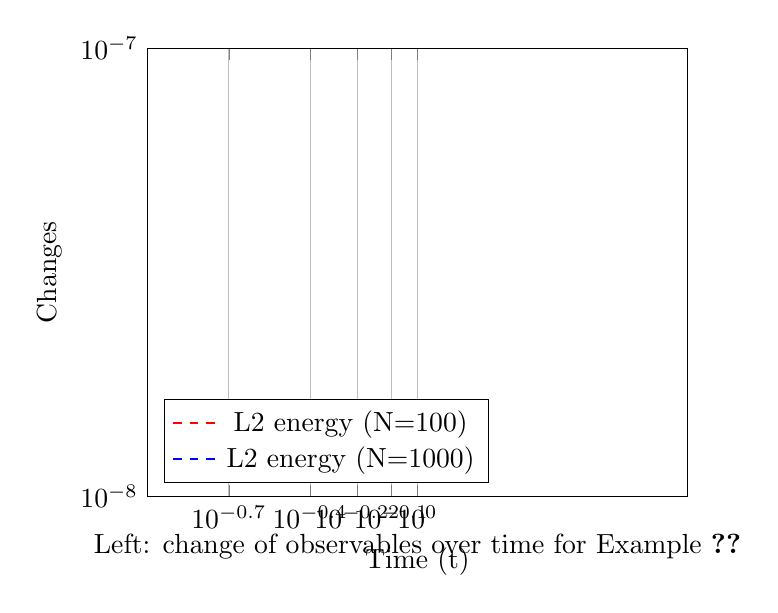
\begin{tikzpicture}
            \begin{loglogaxis}[
                xlabel={Time (t)},
                ylabel={Changes},
                ymin=1e-8, ymax=1e-7,
                xmin=0, xmax=1,
                ytick={1e-8, 1e-7},
                yticklabels={\(10^{-8}\), \(10^{-7}\)},
                xtick={0, 0.2, 0.4, 0.6, 0.8, 1},
                grid=major,
                legend pos=south west,
                log basis x={10},
                log basis y={10},
                title style={at={(0.5,-0.1)}, anchor=north},
                title={Left: change of observables over time for Example \ref{ex: matrix, nonlinear, time-independent}}
            ]
                \addplot[red, dashed] coordinates {(0, 1e-7) (1, 1e-7)};
                \addplot[blue, dashed] coordinates {(0, 1e-7) (1, 1e-7)};
                \legend{L2 energy (N=100), L2 energy (N=1000)}
            \end{loglogaxis}
        \end{tikzpicture}
    \end{minipage}
    \begin{minipage}{0.45\textwidth}
        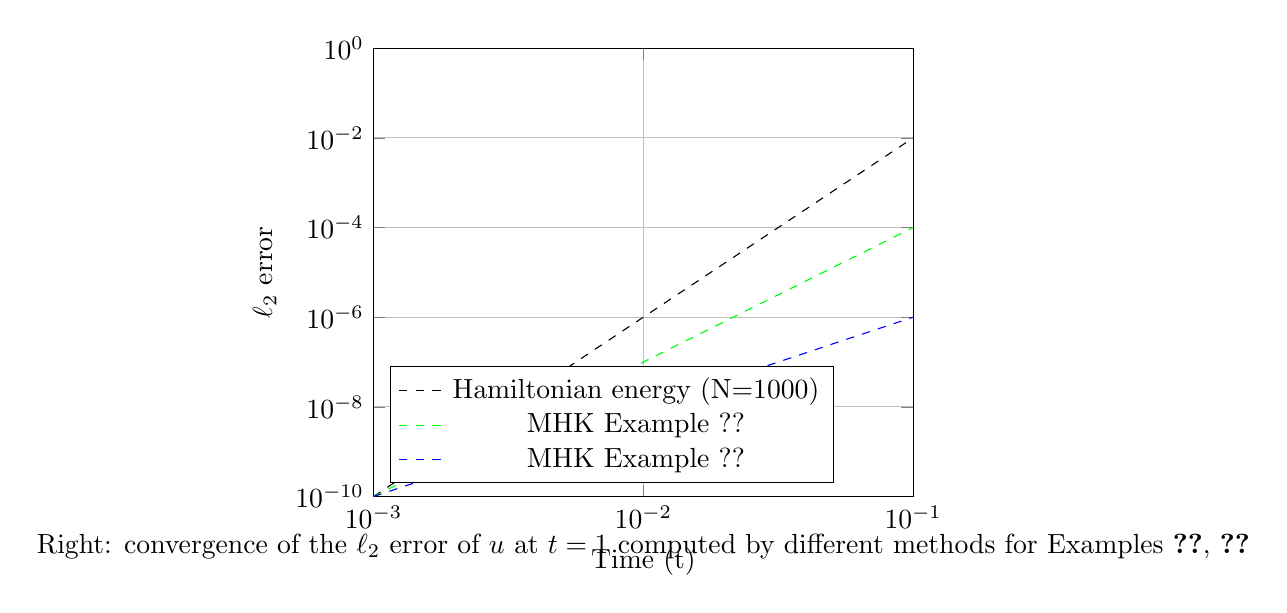
\begin{tikzpicture}
            \begin{loglogaxis}[
                xlabel={Time (t)},
                ylabel={$\ell_2$ error},
                ymin=1e-10, ymax=1e0,
                xmin=1e-3, xmax=1e-1,
                ytick={1e-10, 1e-8, 1e-6, 1e-4, 1e-2, 1e0},
                yticklabels={\(10^{-10}\), \(10^{-8}\), \(10^{-6}\), \(10^{-4}\), \(10^{-2}\), \(10^{0}\)},
                xtick={1e-3, 1e-2, 1e-1},
                grid=major,
                legend pos=south west,
                log basis x={10},
                log basis y={10},
                title style={at={(0.5,-0.1)}, anchor=north},
                title={Right: convergence of the $\ell_2$ error of $u$ at $t = 1$ computed by different methods for Examples \ref{ex: matrix, nonlinear, time-dependent}, \ref{ex: matrix, nonlinear, time-independent}}
            ]
                \addplot[black, dashed] coordinates {(1e-3, 1e-10) (1e-1, 1e-2)};
                \addplot[green, dashed] coordinates {(1e-3, 1e-10) (1e-1, 1e-4)};
                \addplot[blue, dashed] coordinates {(1e-3, 1e-10) (1e-1, 1e-6)};
                \legend{Hamiltonian energy (N=1000), MHK Example ??, MHK Example ??}
            \end{loglogaxis}
        \end{tikzpicture}
    \end{minipage}
\end{figure}

\end{document}